%----------------------------------------------------------------------
% 緒論
%----------------------------------------------------------------------

\chapter{緒論}


\section{Edge Plasmon}

\subsection{文獻回顧}

近幾年，隨著奈米光學與光電元件的快速發展，如何突破傳統光學繞射極限，並將光場限制在極微小的次波長空間內，已成為二維光電元件與光資訊晶片等領域的核心課題。在此背景下，利用一維幾何邊界進行傳導的「邊緣電漿子（Edge Plasmons）」因具備強大的光場限制能力與高微觀動量，成為克服繞射極限並解決動量匹配瓶頸的潛在手段之一。相較於傳統在二維平面傳播的表面電漿極化子（SPPs），邊緣電漿子能將光波波長與場體積進一步壓縮至奈米級的邊緣尺度，在次波長結構邊界處提供顯著的局部場強增強效應，因而被視為在奈米尺度下進行「動量工程」的理想載體。

表面電漿（Surface Plasmons, SPs）的理論研究可追溯至 1957 年由 Ritchie 首次理論預測其在金屬薄膜表面所產生的自由電子集體振盪模態~\cite{ritchie1957plasma}，隨後光學激發與耦合的發展使其延伸為可沿界面傳導的表面電漿極化子（Surface Plasmon Polaritons, SPPs）。然而，邊緣電漿子（Edge Plasmons）這項分支技術的理論起源則為 1988 年，由 Volkov 與 Mikhailov 針對二維電子氣（Two-Dimensional Electron Gas, 2DEG）系統所建立的一維邊緣磁電漿子描述~\cite{volkov1988edge}。該工作在忽略厚度的理想二維極限下，推導出邊緣模式的色散關係與弱阻尼傳播特性，奠定了後續研究的物理起點。在證實邊緣模式的物理基礎後，學術界的研究範式逐漸轉向探討不同結構幾何下的限制規律。2014 年，Schmidt 團隊利用空間解析電子能量損失譜（EELS），量測並分析扁平金屬奈米結構中的邊緣與薄膜模式，並首度提出描述其幾何限制效應的「通用色散關係（Universal Dispersion）」~\cite{schmidt2014}。該研究將扁平結構中複雜的電漿子激發，歸納為邊緣模式與薄膜模式之駐波疊加，並揭示了兩者隨結構尺寸變化的通用色散規律，為後續幾何色散調控的研究提供了物理圖像。

在探索幾何色散規律的同時，邊緣電漿子在實空間的實驗觀測與數值模擬上也取得了突破性進展。2011 年，Gu 等人利用能量過濾穿透式電子顯微鏡（EFTEM）進行實空間成像，首度在單晶金奈米片邊角處捕捉到 wedge-plasmon 反射所形成的共振駐波圖樣~\cite{gu2011resonant}，從實驗上直觀驗證了幾何邊界對電磁波動的局域反射與干涉行為。幾乎在同一時期，邊緣電漿子的研究被迅速引入二維材料系統，Fei 等人於 2015 年利用近場紅外光學顯微鏡（s-SNOM）技術，首度在石墨烯奈米帶邊緣分離並觀測到一維局域化的邊緣電漿子模式~\cite{fei2015edge}，驗證了一維原子邊界對光場極限空間壓縮的物理特性。近年來，研究焦點則朝向主動的色散工程與元件應用，Campos 等人於 2017 年利用掃描穿透式電子顯微鏡結合電子能量損失譜（STEM-EELS）技術映射鋁奈米三角形，成功區分出局域邊緣模式與呼吸模式~\cite{campos2017plasmonic}，展示了幾何截面對場型調製的物理圖像；而另一項研究則利用 q-EELS 技術映射不同厚度之金屬薄膜系統的動量譜線~\cite{shekhar2017momentum}，證實了僅需改變金屬幾何厚度即可調控電漿子的色散關係。這項關於幾何厚度相依性的物理規律，直接為利用一維邊緣限制進行動量匹配與二維材料量子元件的開發，提供了重要的實驗對照依據。

\begin{table}[H]  % 結合強制定位
	\centering
	\footnotesize % 微調字體大小，縮小體積以利排版
	\captionsetup{labelsep=quad, name=TABLE}
	\renewcommand{\arraystretch}{1.4} % 透過調整行高取代手動加空行，空間利用更精準
	
	\begin{tabular}{r | p{11cm}}
		\hline\hline
		1988 & Volkov 與 Mikhailov 針對二維電子氣（2DEG），在忽略厚度的極限下理論推導出邊緣磁電漿子（Edge Magnetoplasmons）的色散關係與弱阻尼特性~\cite{volkov1988edge}。 \\
		2011 & Gu 等人利用 EFTEM 實空間成像結合 FDTD 模擬，在單晶金奈米片邊角處觀測到楔形電漿子（Wedge-Plasmon）反射所形成的共振駐波圖樣~\cite{gu2011resonant}。 \\
		2014 & Schmidt 等人利用 EELS 技術量測扁平金屬奈米結構，將模式分解為邊緣與薄膜模式之駐波疊加，並提出通用色散關係（Universal Dispersion）~\cite{schmidt2014}。 \\
		2015 & Fei 等人利用 s-SNOM 技術，在石墨烯奈米帶邊緣首度以實空間成像分離並觀測到一維局域化的邊緣電漿子（1D Edge Plasmons）模式~\cite{fei2015edge}。 \\
		2017 & Campos 等人利用 STEM-EELS 技術，在鋁奈米三角形中成功區分並定位了局域於結構邊緣的邊緣模式（Edge Modes）~\cite{campos2017plasmonic}。 \\
		2017 & Shekhar 等人利用 q-EELS 技術映射金屬薄膜（Thin Films）的動量色散關係，證實改變金屬幾何厚度可調控電漿子色散，為理解邊緣模式的厚度效應提供對照依據~\cite{shekhar2017momentum}。 \\
		\hline\hline
	\end{tabular}
	\vspace{0.3cm}
	
	\caption{edge plasmon 發展年表}
	\label{tab:edge_plasmon_history}
\end{table}

\subsection{Edge Plasmon 物理機制}

邊緣電漿子（Edge Plasmon）的物理本質，是局域於導電薄膜或二維材料幾何邊界處的集體電子共振振盪行為。與一般在無限平面上傳播的表面電漿子（Surface Plasmon Polaritons, SPPs）不同，邊緣電漿子的存在完全取決於結構在空間中的不連續性。當外加電磁場激發結構時，由於金屬介質與介電材料的交界面形貌發生劇烈突變，自由電荷會在邊緣局部大量堆積，進而形成沿著一維邊界線傳播、且在垂直邊界方向呈指數級衰減的局域化電磁模式~\cite{volkov1988edge}。

從色散關係與幾何效應的角度來看，邊緣電漿子的特性高度依賴於薄膜的厚度與邊界形狀。當金屬薄膜的厚度縮減至奈米級極限時，空間限制效應會使得邊緣處的有效電荷密度分佈發生改變，導致其傳播波向量（Wavevector）顯著大於同頻率下的自由空間光子，這賦予了邊緣電漿子將光場限制在極小奈米尺度內的能力~\cite{schmidt2014, shekhar2017momentum}。同時，結構的截面形狀（例如垂直切面邊緣）會直接影響局部電荷的分布密度，使得邊緣電漿子的共振頻率通常低於傳統的表面電漿子，展現出獨特的準一維色散限制規律~\cite{gu2011resonant}。這種因幾何截斷而誘發的高局部場強增強效應與色散調諧特性，使其成為探測局域光交互作用與材料特性的理想工具。
\begin{figure}[H]
	\centering
	% (a) 金屬架構示意圖
	\begin{subfigure}[b]{0.32\textwidth}
		\centering
		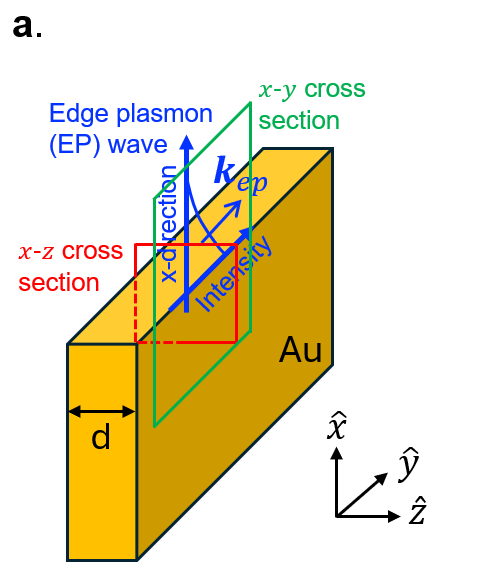
\includegraphics[width=\textwidth]{Figures/edge plasmon金屬架構示意圖}
		\caption{架構示意圖}
		\label{fig:ep_sub_a}
	\end{subfigure}
	\hfill
	% (b) edge plasmon(1)
	\begin{subfigure}[b]{0.32\textwidth}
		\centering
		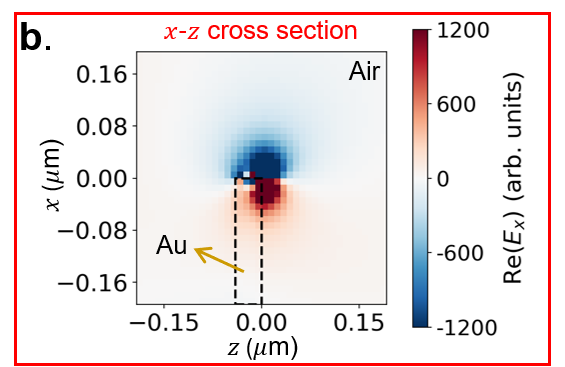
\includegraphics[width=\textwidth]{Figures/edge plasmon(1)}
		\caption{$x-z$ cross section}
		\label{fig:ep_sub_b}
	\end{subfigure}
	\hfill
	% (c) edge plasmon(2)
	\begin{subfigure}[b]{0.32\textwidth}
		\centering
		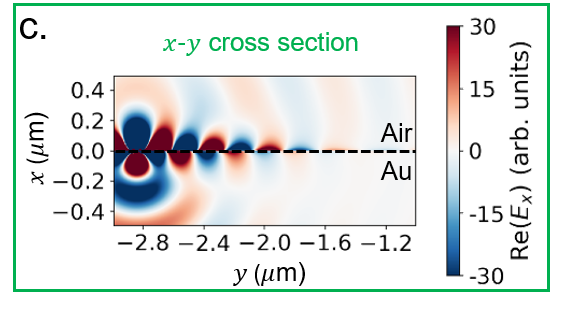
\includegraphics[width=\textwidth]{Figures/edge plasmon(2)}
		\caption{$x-y$ cross section}
		\label{fig:ep_sub_c}
	\end{subfigure}
	
\caption{金屬薄膜邊緣電漿（Edge Plasmons）之一維傳播與局域特性：(a) 模態傳播之幾何架構示意圖；(b) 局域於金屬邊緣之 $x-z$ 切面電場強度 $\mathrm{Re}(E_x)$ 分佈，顯示其次波長局域效應；(c) 沿邊緣傳播方向之 $x-y$ 切面電場分佈，展現其一維（1D）導波特性。}
\label{fig:edge_plasmon_group}
\end{figure}
\section{過渡金屬二硫族化合物（TMDs）}

\subsection{文獻回顧}
過渡金屬二硫族化合物（Transition Metal Dichalcogenides, TMDs）在單原子層厚度下展現出獨特的能帶結構與強烈的激子物理效應，在次波長光電元件與低維度光子學的設計中展現出關鍵的應用潛力。

單層 TMDs 的實驗光譜研究可追溯至 2010 年，由 Mak 等人~\cite{mak2010}與 Splendiani 等人~\cite{splendiani2010}在實驗上首次證實單層二硫化鉬（$\text{MoS}_2$）具備直接能隙（Direct Bandgap）。此一發現證實了單層材料相較於間接能隙的塊材，具備顯著提升的光學發光效率，促進了後續二維半導體元件的發展。在材料能帶結構確立後，研究焦點進一步轉向其特有的對稱性破缺特性。Xiao 等人於 2012 年從空間反演對稱性破缺出發，理論奠定了單層 TMDs 中的自旋-谷鎖定（Spin-Valley Locking）與谷選擇光學躍遷定則~\cite{xiao2012}，為光學主動控制二維量子態提供了物理機制。

與此同時，由於二維材料在垂直方向的量子限制效應，使得激子（Exciton）效應在 TMDs 的光譜中佔據主導地位。2015 年，Qiu 等人利用第一性原理 GW-BSE 計算指出，單層 TMDs 中的亮激子（Bright Exciton）在布里淵區中心附近，因長程電子-電洞交換作用會產生非解析的線性色散行為，其特徵與光子極其相似，因而被定義為「類光（Light-like）激子色散」~\cite{qiu2015}。該工作指出單層 TMDs 中的亮激子色散偏離了傳統半導體中的拋物線二次色散（$E \propto Q^2$）關係，為探討低維度系統下的激子輸送與非線性散射機制提供了理論框架。

然而，此類具備極大群速度的高動量激子在傳統光學探測中，面臨著光子動量過小而難以直接激發的動量失配（Momentum mismatch）瓶頸。為了在實驗中探測並控制這類有限動量的激子，Simbulan 等人於 2021 年利用帶軌道角動量（OAM）的扭曲光（Twisted Light）進行光學激發~\cite{simbulan2021}，透過光譜的非線性藍移，首次在實驗上證實了單層 $\text{MoS}_2$ 激子的類光色散關係。儘管扭曲光提供了選擇性激發有限動量激子的手段，但如何在固態晶片上實現微觀尺度的動量工程，依然是二維光電元件整合上難以跨越的技術難題。

為了突破此一固態晶片上的整合瓶頸，近年來，利用具備高微觀動量的金屬邊緣電漿（Edge Plasmons）與 TMDs 激子色散進行共振耦合，被提出作為在晶片上實現次波長尺度下動量工程（Momentum engineering）的潛在解決方案。

\begin{table}[H]  % 結合強制定位
	\centering
	\footnotesize % 微調字體大小，縮小體積以利排版
	\captionsetup{labelsep=quad, name=TABLE}
	\renewcommand{\arraystretch}{1.4} % 透過調整行高優化空間
	
	\begin{tabular}{r | p{11cm}}
		\hline\hline
		2010 & Mak 等人與 Splendiani 等人首度在實驗上證實單層二硫化鉬（$\text{MoS}_2$）具備直接能隙特徵，展現強烈的光學發光效率~\cite{mak2010, splendiani2010}。 \\
		2012 & Xiao 等人理論奠定了單層 TMDs 中的自旋-谷鎖定與谷選擇光學躍遷定則，為谷電子學提供了核心物理基礎~\cite{xiao2012}。 \\
		2015 & Qiu 等人理論預測單層 TMDs 中的激子在中心動量附近，因長程交換作用而產生非解析的線性「類光（Light-like）」色散關係~\cite{qiu2015}。 \\
		2021 & Simbulan 等人利用帶軌道角動量的扭曲光（Twisted Light）進行光學激發，在實驗上證實了單層 $\text{MoS}_2$ 激子的類光色散關係~\cite{simbulan2021}。 \\
		\hline\hline
	\end{tabular}
	\vspace{0.3cm}
	
	\caption{TMD 激子物理發展年表}
	\label{tab:tmd_exciton_history}
\end{table}

\subsection{TMD 材料特性與能帶結構}
過渡金屬二硫族化合物的化學式通常寫作 $\text{MX}_2$（其中 $\text{M}$ 代表鉬 $\text{Mo}$ 或鎢 $\text{W}$ 等過渡金屬；$\text{X}$ 代表硫 $\text{S}$、硒 $\text{Se}$ 或碲 $\text{Te}$ 等硫屬元素）。在晶體結構上，單層 TMDs 呈現三明治狀態的三原子層夾心排列，中間的單層過渡金屬原子與上下兩層的硫屬原子以強烈的共價鍵緊密結合；其中，具備六方晶格對稱性的組態在結構上最為穩定，亦是展現二維半導體量子特性的核心幾何特徵。

\begin{figure}[H]
	\centering
	% (a) TMD 俯視圖
	\begin{subfigure}[b]{0.6\textwidth}
		\centering
		
\includegraphics[width=\textwidth]{tmd_top_view}
		\caption{Top view}
		\label{fig:tmd_structure_a}
	\end{subfigure}
	
	% 這裡故意空一行，LaTeX 就會自動換行把下一張圖放到下方
	
	% (b) TMD 側視圖
	\begin{subfigure}[b]{0.6\textwidth}
		\centering
		
\includegraphics[width=\textwidth]{tmd_side_view}
		\caption{Side view}
		\label{fig:tmd_structure_b}
	\end{subfigure}
	
	\caption{單層過渡金屬二硫族化合物（TMD）之晶體結構示意圖。(a) 俯視圖（Top view），展現由過渡金屬原子 M 與硫族原子 X 組成之蜂巢狀晶格；(b) 側視圖（Side view），顯現 X-M-X 的三原子層夾心結構。}
	\label{fig:tmd_crystal_structure}
\end{figure}

當 TMDs 的材料厚度由三維塊材（Bulk）減少至單層（Monolayer）時，由於量子限制效應與層間耦合逐漸減弱，其能帶結構會發生顯著變化~\cite{splendiani2010, mak2010}。在塊材狀態下，材料呈現間接能隙（Indirect Bandgap）特徵，而位於第一布里淵區角落 $K$（及其等價的 $K'$）點的直接能隙雖然存在，但其能量高於間接能隙，因此並非材料的最低能隙~\cite{mak2010}。隨著材料厚度降低，層間凡德瓦耦合逐漸消失，使與間接躍遷相關的能帶位置發生明顯改變，導致間接能隙逐漸增大；相較之下，$K$ 點的直接能隙變化較小。當材料減薄至單層時，直接能隙成為最低能隙，使材料由間接能隙半導體轉變為直接能隙半導體~\cite{splendiani2010, mak2010}。在此情況下，電子與電洞可於相同動量空間位置進行輻射複合，無需額外聲子（Phonon）參與以滿足動量守恆，因此大幅提升了材料的光吸收與發光效率。

此外，當材料減薄至單層後，由於空間反演對稱性（Inversion Symmetry）破缺，強烈的自旋-軌道耦合（Spin-Orbit Coupling, SOC）會導致能帶產生顯著的自旋分裂，使第一布里淵區角落的 $K$ 與 $K'$ 谷在價帶頂部形成谷對比自旋分裂（Valley-Contrasting Spin Splitting）~\cite{xiao2012}。受到時間反演對稱性（Time-Reversal Symmetry）的限制，$K$ 谷與 $K'$ 谷對應的價帶頂部具有相反的自旋取向，形成特有的自旋-谷鎖定（Spin-Valley Locking）效應~\cite{xiao2012}。此一能帶特徵進一步決定了谷相依光學選擇定則（Valley-Dependent Optical Selection Rules），使 $K$ 與 $K'$ 谷的激子分別選擇性地與右旋（$\sigma^+$）及左旋（$\sigma^-$）圓偏振光耦合~\cite{xiao2012, mak2012control}。因此，可藉由圓偏振光激發特定谷中的載子與激子態，進而以純光學方式主動操控材料的谷自由度（Valley Degree of Freedom）~\cite{mak2012control}。

\begin{figure}[H]
	\centering
	
	% 上方：四組谷的能帶結構圖 (different vally.png)
	\begin{minipage}[b]{0.85\textwidth}
		\centering
		
\includegraphics[width=\textwidth]{different vally}
		\vspace{0.1cm} 
	\end{minipage}
	
	% 💡 這裡故意空一行自動換行
	
	% 下方：第一布里淵區六邊形 (TMD_BZ.png)
	\begin{minipage}[b]{0.38\textwidth} 
		\centering
		
\includegraphics[width=\textwidth]{TMD_BZ}
	\end{minipage}
	
	% 3. 統一的精簡圖說
	\caption{單層過渡金屬二硫族化合物（TMD）之谷能帶結構與布里淵區示意圖。上方左側為鎢系材料（$\text{WSe}_2, \text{WS}_2$）與右側為鉬系材料（$\text{MoSe}_2, \text{MoS}_2$）於 $K$ 與 $K'$ 谷之能帶自旋分裂及光學選擇定則；下方為對應之六方第一布里淵區幾何示意圖。}
	\label{fig:tmd_spin_valley_locking_combined}
\end{figure}

\subsection{TMD 激子色散關係與類光特性（Light-like）}
在單層 TMDs 中，由於材料僅具有原子級厚度，其上下介電環境產生明顯不連續性，使二維系統中的介電屏蔽效應大幅減弱。再加上二維量子侷限效應的影響，電子與電洞之間的庫侖作用顯著增強，形成具有數百毫電子伏特結合能的穩定激子（Exciton）態；其結合能遠高於室溫熱能（約 26~meV），因此即使在室溫下仍能穩定存在。

在單層 TMDs 的激子能帶結構中，激子能量隨質心動量 $Q$ 的變化關係在 $Q \approx 0$ 附近呈現特殊的非解析行為。不同於傳統半導體激子主要由有限有效質量所主導的拋物線色散，單層 TMD 中的谷激子受到長程電子-電洞交換作用（Long-range Electron-Hole Exchange Interaction）影響，在原有拋物線色散基礎上引入與 $|Q|$成正比的非解析項，使色散在小動量區域呈現近似線性的分裂特徵~\cite{qiu2015}。由於此線性分支與自由光子的線性色散形式相似，因此本文將其稱為類光（Light-like）激子色散。

然而，只有極接近 $Q = 0$ 的激子態位於光錐（Light Cone）內並能與自由空間光有效耦合，而大部分具有有限動量的類光激子則位於光錐之外。由於自由空間光子的面內動量極小，在光學激發上無法跨越巨大的動量失配，導致外界光子難以直接與這些高動量的激子狀態產生共振匹配。儘管在實驗上可利用帶軌道角動量的扭曲光（Twisted Light）提供選擇性激發以匹配部分有限動量~\cite{simbulan2021}，但在固態晶片整合與主動調控上依然面臨極大瓶頸。因此，尋找兼具微觀尺度光場侷限與大動量特徵的傳導模式，已成為當前重要的研究課題。
\section{研究動機}
雖然透過外部構造光場（如扭曲光）能為單層過渡金屬二硫族化合物（TMDs）注入特定的空間相位分佈，從而開闢激發有限動量激子的通道，然而這類光學調控方式所能提供的波向量仍局限於光錐（Light cone）附近的低動量區域，在探測與激發高動量空間（k-space）量子態的能力上存在物理極限~\cite{simbulan2021}。相較之下，利用導電薄膜幾何邊緣所誘發的邊緣電漿子（Edge plasmons），因其具備強烈的光場局域化效應與超越自由空間光學極限的高微觀動量，是進行微觀動量匹配的有效載體。

若要利用邊緣電漿子激發或點亮單層 TMDs 的高動量激子態，核心關鍵在於使電漿子的幾何色散曲線與單層 TMDs 獨特的類光（Light-like）激子色散關係在動量空間中產生共振交點。此交點在物理上代表能量與動量同時滿足守恆條件的窗口；在此共振行為下，費米黃金律（Fermi's golden rule）中的躍遷矩陣元將獲得極大化，從而克服動量失配並提升光學躍遷速率。然而，此邊緣電漿子模式的幾何色散關係隨金屬薄膜厚度變化的相依性與變化規律，目前仍缺乏系統性的數值模擬與定量分析。

基於上述物理機制，本研究利用時域有限差分法（FDTD），透過開源模擬軟體 MEEP~\cite{oskooi2010meep}，探討金屬薄膜厚度對邊緣電漿子模式色散曲線的調控效應。本工作聚焦於動量空間中色散曲線交點的變化趨勢，透過模擬證實，當金屬薄膜厚度減少時，邊緣電漿子模式的色散關係將趨於壓平，使其與單層 TMDs 色散關係的共振交點往高動量區（High-momentum regime）移動。本工作闡明了薄膜厚度對共振匹配位置的幾何調控規律，研究結果可為未來二維材料基光電與量子元件的結構設計提供具體的物理依據。